\documentclass[tikz,border=12pt]{standalone}
\usepackage[T1]{fontenc}
\usepackage{lmodern,amsmath,amssymb}
\usetikzlibrary{arrows.meta,positioning,calc}
\definecolor{ink}{HTML}{183444}
\definecolor{blue}{HTML}{1B6780}
\definecolor{amber}{HTML}{AD601A}
\begin{document}
\hyphenpenalty=10000\exhyphenpenalty=10000
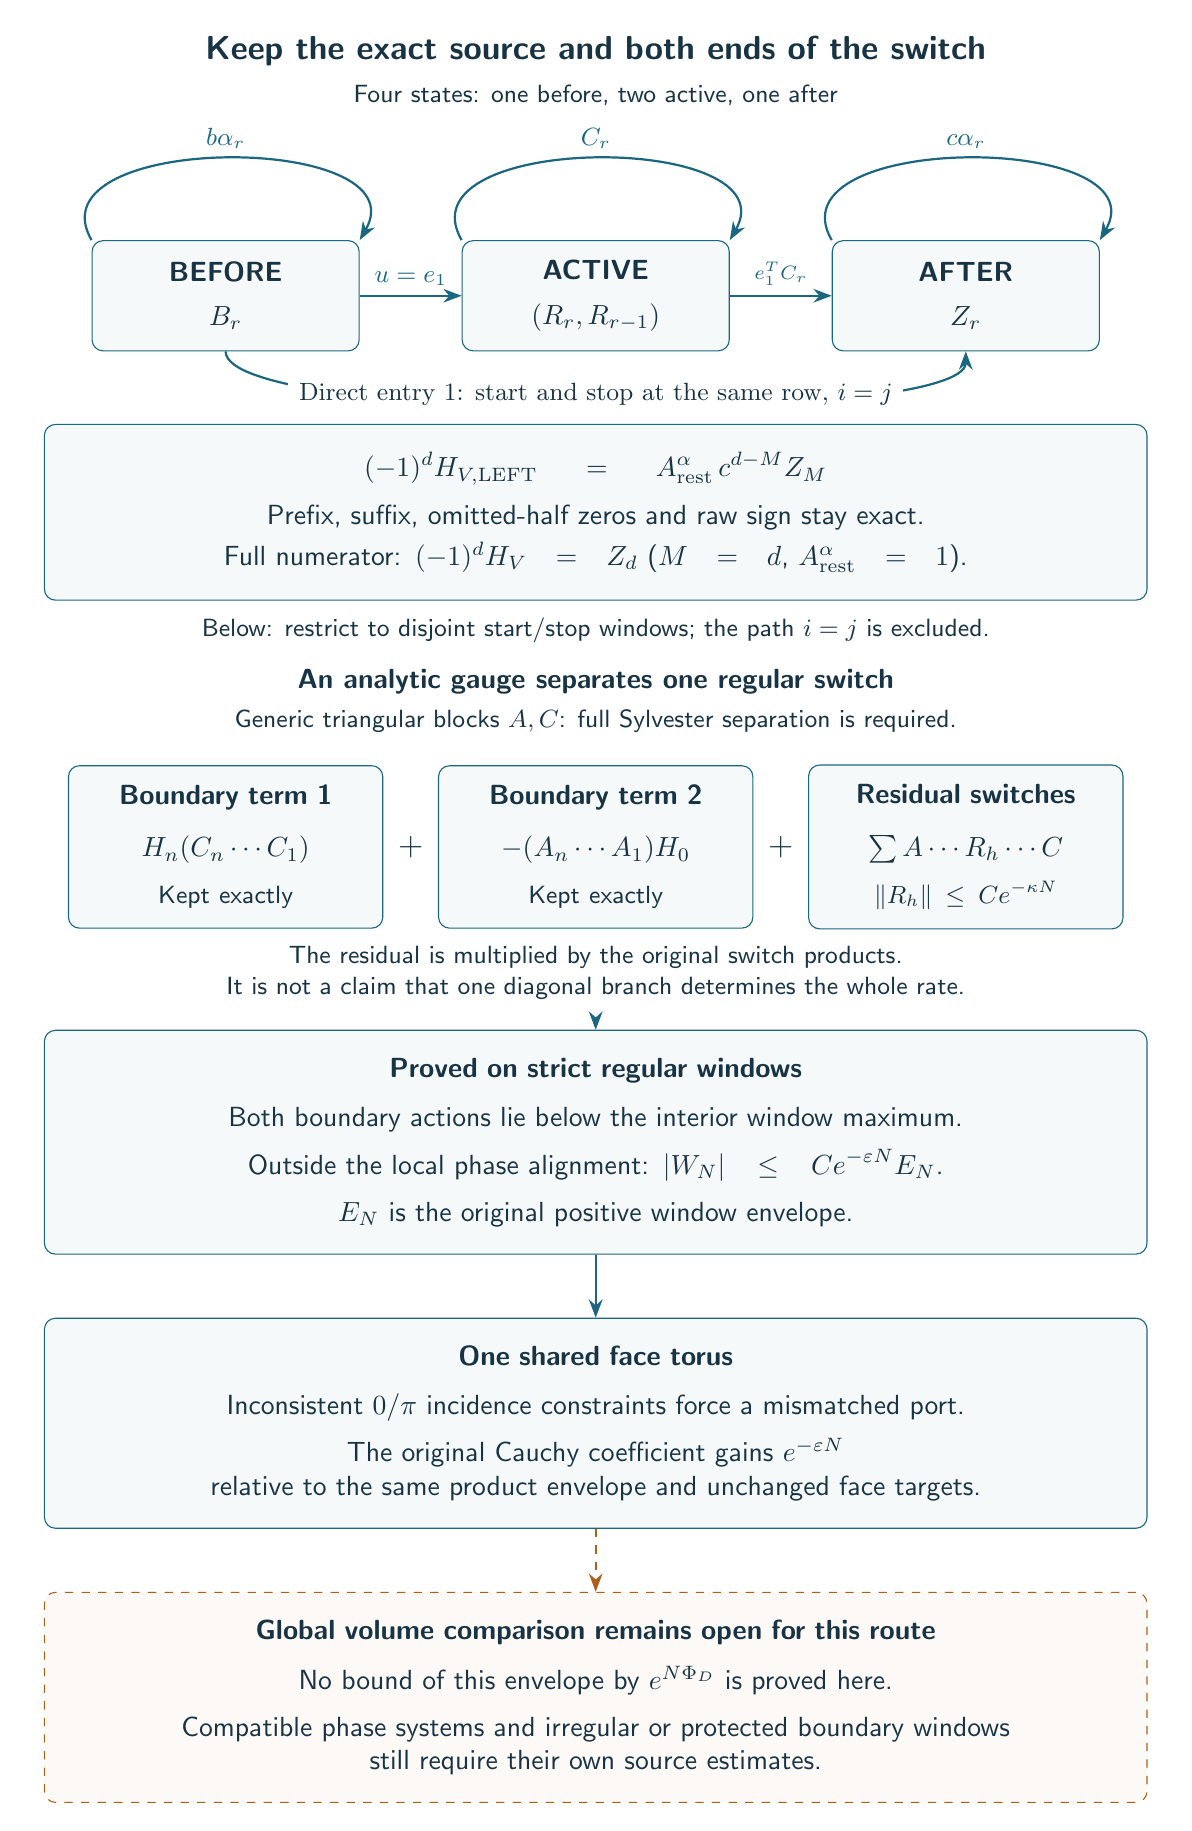
\begin{tikzpicture}[font=\sffamily,text=ink,>=Stealth,
 state/.style={draw=blue,fill=blue!4,rounded corners,align=center,
               minimum height=14mm,text width=29mm,inner sep=7pt},
 panel/.style={draw=blue,fill=blue!4,rounded corners,align=center,
               text width=13.3cm,inner sep=10pt},
 term/.style={panel,text width=35mm,minimum height=19mm,inner sep=7pt},
 pending/.style={panel,draw=amber,fill=amber!4,dashed}]
\node[font=\sffamily\large\bfseries] at (0,3.1) {Keep the exact source and both ends of the switch};
\node[font=\sffamily\small] at (0,2.55) {Four states: one before, two active, one after};
\node[state] (before) at (-4.7,0) {\textbf{BEFORE}\\[4pt]$B_r$};
\node[state] (active) at (0,0) {\textbf{ACTIVE}\\[4pt]$(R_r,R_{r-1})$};
\node[state] (after) at (4.7,0) {\textbf{AFTER}\\[4pt]$Z_r$};
\draw[->,thick,blue] (before) -- node[above,font=\small] {$u=e_1$} (active);
\draw[->,thick,blue] (active) -- node[above,font=\scriptsize] {$e_1^TC_r$} (after);
\draw[->,thick,blue] (before.north west) to[out=120,in=60,looseness=1.2]
 node[above,font=\small] {$b\alpha_r$} (before.north east);
\draw[->,thick,blue] (active.north west) to[out=120,in=60,looseness=1.2]
 node[above,font=\small] {$C_r$} (active.north east);
\draw[->,thick,blue] (after.north west) to[out=120,in=60,looseness=1.2]
 node[above,font=\small] {$c\alpha_r$} (after.north east);
\draw[->,thick,blue] (before.south) .. controls (-4.7,-1.65) and (4.7,-1.65)
 .. (after.south);
\node[fill=white,inner sep=4pt,font=\small] at (0,-1.25)
 {Direct entry $1$: start and stop at the same row, $i=j$};
\node[panel] at (0,-2.75) {
 $\displaystyle (-1)^dH_{V,\mathrm{LEFT}}
       =A_{\mathrm{rest}}^\alpha\,c^{d-M}Z_M$\\[5pt]
 Prefix, suffix, omitted-half zeros and raw sign stay exact.\\[3pt]
 Full numerator: $(-1)^dH_V=Z_d$ ($M=d$, $A_{\mathrm{rest}}^\alpha=1$).};
\node[font=\sffamily\small] at (0,-4.25)
 {Below: restrict to disjoint start/stop windows; the path $i=j$ is excluded.};

\node[font=\sffamily\bfseries] at (0,-4.9) {An analytic gauge separates one regular switch};
\node[font=\sffamily\small] at (0,-5.4)
 {Generic triangular blocks $A,C$: full Sylvester separation is required.};
\node[term] (leftterm) at (-4.7,-7.0)
 {\textbf{Boundary term 1}\\[7pt]$H_n(C_n\cdots C_1)$\\[5pt]\small Kept exactly};
\node[term] (rightterm) at (0,-7.0)
 {\textbf{Boundary term 2}\\[7pt]$-(A_n\cdots A_1)H_0$\\[5pt]\small Kept exactly};
\node[term] (residual) at (4.7,-7.0)
 {\textbf{Residual switches}\\[7pt]$\sum A\cdots R_h\cdots C$\\[5pt]\small $\|R_h\|\le Ce^{-\kappa N}$};
\node[font=\large] at (-2.35,-7.0) {$+$};
\node[font=\large] at (2.35,-7.0) {$+$};
\node[font=\sffamily\small,align=center] at (0,-8.6)
 {The residual is multiplied by the original switch products.\\
 It is not a claim that one diagonal branch determines the whole rate.};

\node[panel] (window) at (0,-10.75)
 {\textbf{Proved on strict regular windows}\\[6pt]
 Both boundary actions lie below the interior window maximum.\\[5pt]
 Outside the local phase alignment:
 $\displaystyle |W_N|\le Ce^{-\varepsilon N}E_N$.\\[5pt]
 $E_N$ is the original positive window envelope.};
\draw[->,thick,blue] (0,-9.2)--(window.north);
\node[panel,below=8mm of window] (shared)
 {\textbf{One shared face torus}\\[6pt]
 Inconsistent $0/\pi$ incidence constraints force a mismatched port.\\[5pt]
 The original Cauchy coefficient gains $e^{-\varepsilon N}$\\
 relative to the same product envelope and unchanged face targets.};
\draw[->,thick,blue] (window.south)--(shared.north);
\node[pending,below=8mm of shared] (open)
 {\textbf{Global volume comparison remains open for this route}\\[6pt]
 No bound of this envelope by $e^{N\Phi_D}$ is proved here.\\[5pt]
 Compatible phase systems and irregular or protected boundary windows\\
 still require their own source estimates.};
\draw[->,thick,amber,dashed] (shared.south)--(open.north);
\end{tikzpicture}
\end{document}
